\documentclass[10pt]{article}

\usepackage{amsmath}
\usepackage{amsfonts}
\usepackage{amssymb}
\usepackage{graphicx}
\usepackage{xcolor}
\usepackage{tikz}

\begin{document}
\section{Saját parancsok}
\newcommand{\ossz}[2]{#1 + #2 =}
\newcommand{\kiv}[2]{#1 - #2 =}
\ossz{2}{5} \\
\ossz{10}{16} \\
\kiv{9}{8} \\

\newcommand{\numpad}{\begin{tabular}{ccc}
7&8&9\\
4&5&6\\
1&2&3
\end{tabular}}

\numpad\\

\newcommand{\R}{$\mathbb{R}$}

\R

\section{Grafika}
\begin{center}
\includegraphics[scale=0.5]{C:/Bence/sje/Selye_logo.png}
\end{center}

\subsection{Színezés}
\color{blue}
kék
\color{black}
fekete\\
\textcolor{red}{piros piros piros}
fekete fekete fekete
\textcolor{cyan}{haha}
\colorbox{cyan}{haha}
\pagecolor{orange!50}
\begin{center}
\includegraphics[scale=0.4]{C:/Bence/sje/latex-colors.png}
\end{center}

\definecolor{cc1}{rgb}{0.5,0.2,0.6}
\definecolor{cc2}{RGB}{127,35,65}
\definecolor{cc3}{HTML}{32CD32}
\textcolor{cc1}{sajat szin}\\
\textcolor{cc2}{sajat szin}\\
\textcolor{cc3}{sajat szin}\\

\section{Rajzolás}

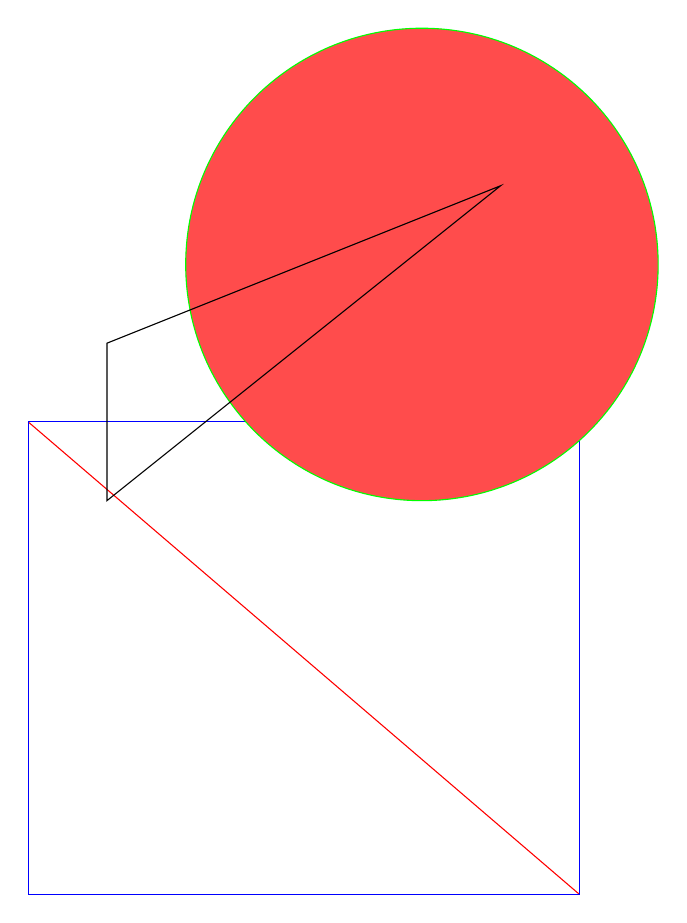
\begin{tikzpicture}
%\draw (-1, 2) -- (8, -6);
\draw[red] (-1, 2) -- (6, -4);

\draw[blue](-1,2) rectangle (6,-4);

\filldraw[color=green, fill=red!70] (4,4) circle (3);

\draw (0,1) -- (0,3) -- (5,5) -- cycle;

\end{tikzpicture}
\newpage
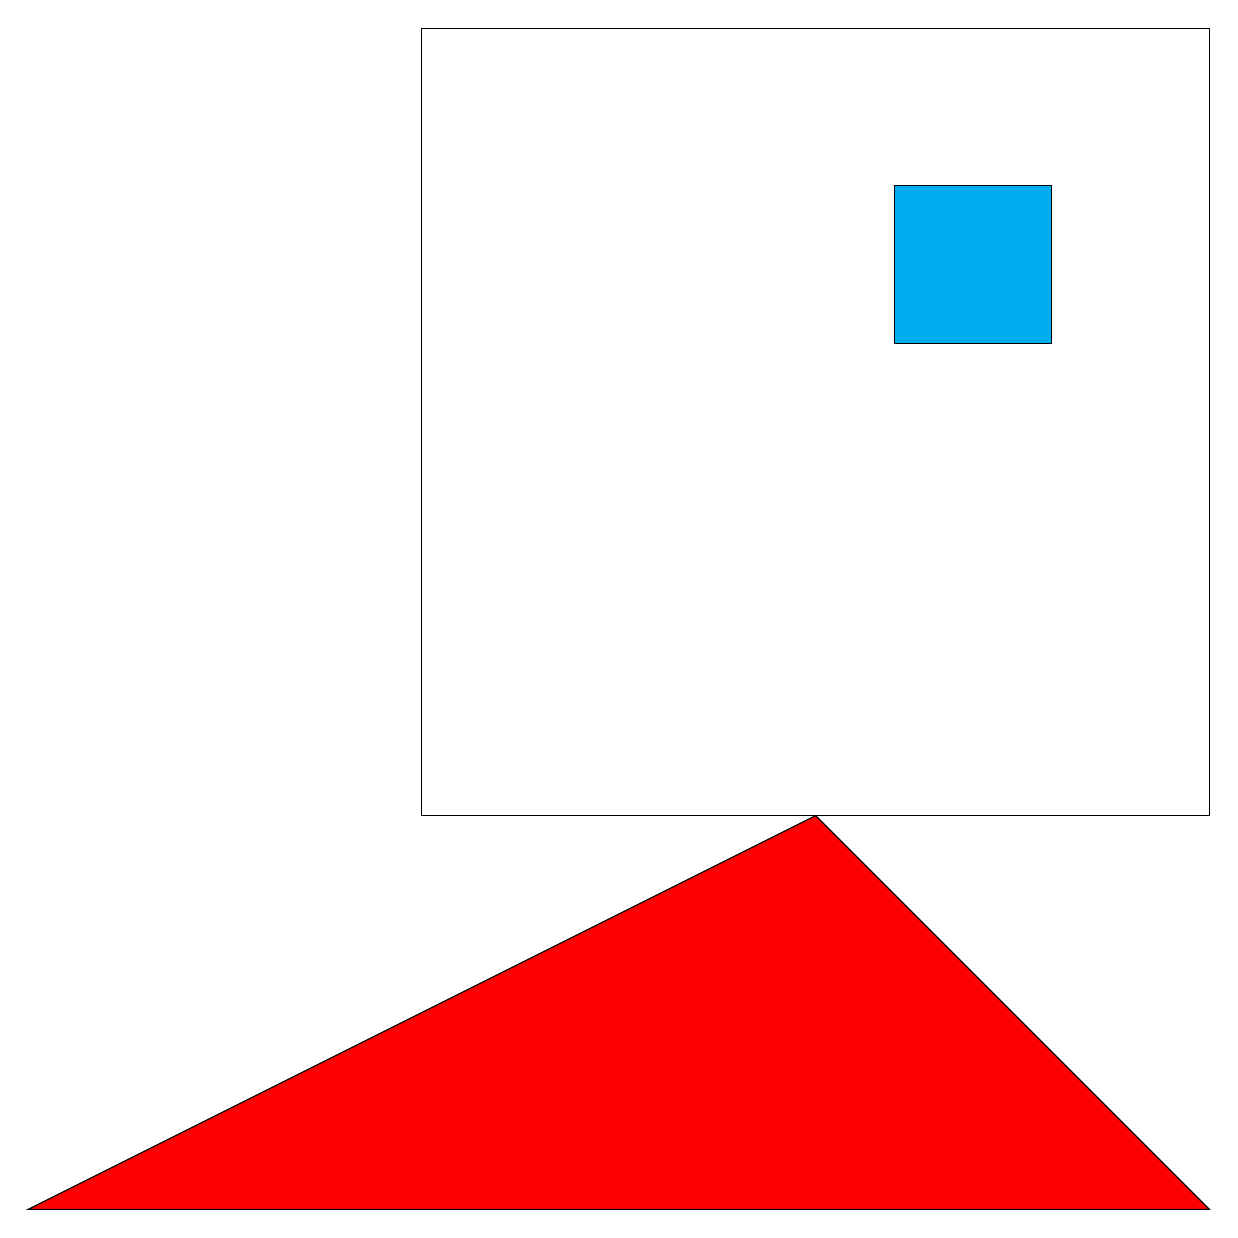
\begin{tikzpicture}
\filldraw[color=black,fill=white] (0,0) rectangle (10,10);
\filldraw[color=black,fill=cyan] (6,6) rectangle (8,8);
\filldraw[color=black,fill=red] (5,0) -- (10,-5) -- (-5,-5) -- cycle;
\end{tikzpicture}
\end{document}